\documentclass[preprint,titlepage,preprintnumbers,amsmath,amssymb,aps,11pt]{revtex4-2}

\usepackage[utf8]{inputenc}  % UTF-8 enabled
\usepackage{graphicx}  % Include figure files
\usepackage{xcolor}  % Allow for a color text
\usepackage{amsmath}  % math fonts
\usepackage{amsfonts}  % math fonts
\usepackage{latexsym}  % math fonts
\usepackage{amssymb}  % math fonts
\usepackage{bm}  % bold math fonts
\usepackage{hyperref}  % add hypertext capabilities
\usepackage{setspace}
\usepackage{listings}

\graphicspath{ {images/} }

\begin{document}

\preprint{\textcolor{red}{PHYS-304:} Fall 2020}
\title{Modeling Dynamics of Euler's Three Body Problem}
\author{Jasper Swallen}
\affiliation{
    Department of Physics and Astronomy, University of Southern California,
    Los Angeles, California 90089, USA
}
\date{\today}


\begin{abstract}
    Euler's Three Body Problem is a simplification of the general 3-Body Problem, with two fixed large masses and one free mass. While it is possible to solve Euler's Three Body Problem analytically, the solutions are not simple to evaluate in Cartesian coordinates. Instead, various numerical methods were used. Euler's method, the Runge-Kutta method, and Forest \& Neri's method were used. With these methods, plots were generated in Python based on various initial conditions. Forest \& Neri's method was found to be the most precise, followed by Runge-Kutta and then Euler's Method. Euler's Method had the fastest runtime, followed by Forest \& Neri and then the Runge-Kutta methods.
        {\singlespacing \tableofcontents}
\end{abstract}

\maketitle


\section{Background and Applications}
Euler's Three Body Problem is a simplification of the 3-body problem (which is itself a special case of the $N$-body problem). The general $N$-body problem is to describe the movement of $N$ masses which exert an attractive gravitational force on each other. In Euler's simplification, two large bodies are fixed at points in space (and are assumed to not act upon each other), while one smaller body is free to move through space. This smaller body's movement is dependent only on its relative position to the two larger masses and their masses. It can be assumed that the smaller mass $m$ is much smaller than the two larger masses $m_2$ and $m_3$. This can therefore be represented by a one-body problem. Given the level of simplification, it would not seem that this system is a close representation of real-world problems. However, this is not the case.

There are two main applications of this problem. In our solar system, this is a very close representation of the movement of comets which interact with Jupiter and the sun \cite{Worthington2012,Koon2000}. The other application is in an electric field. Although electric fields are not described by exactly the same forces, their potential is still inverse to the distance. Thus, an analogue would be an electron moving through the electric field of two nuclei.

\begin{figure}
    \centering
    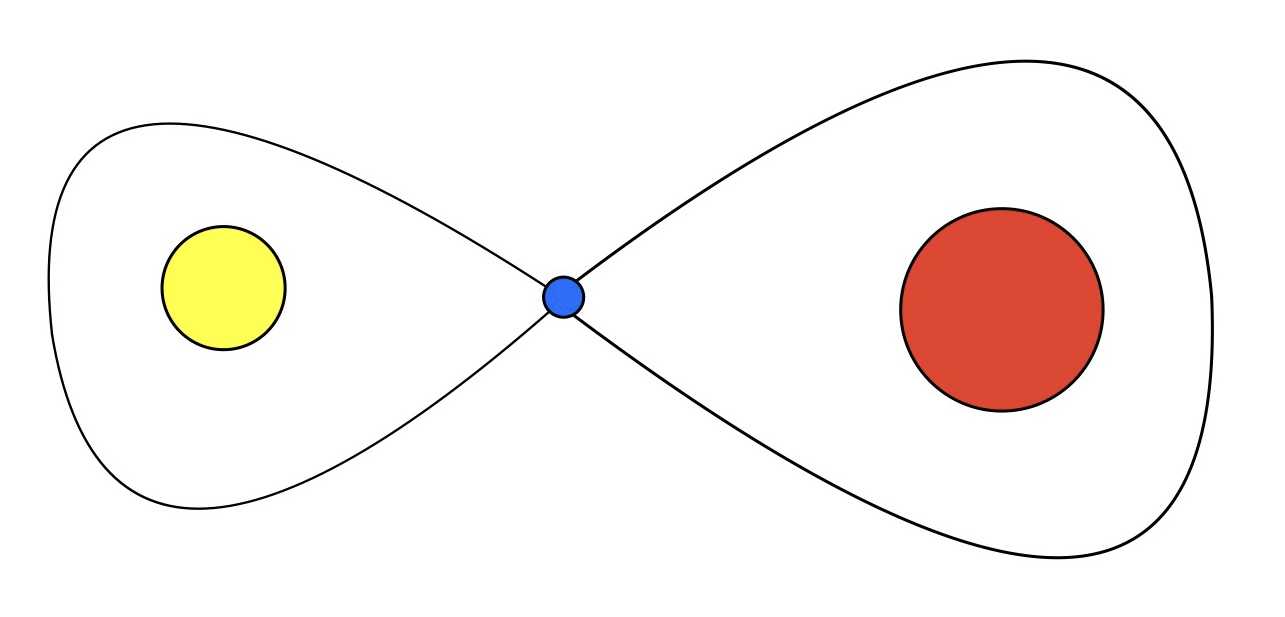
\includegraphics[width=0.5\textwidth]{Fig 1.jpeg}
    \caption{A model solar system with simplified orbits}
    \label{fig:orbit}
\end{figure}

To solve $N$-body problems, the gravitational forces must be known. Newton's Law of Gravitation states that, for any two masses $m_1$ and $m_2$ separated by a radius $r=|\bm{r_1}-\bm{r_2}|$ (where $\bm{r_1}$ and $\bm{r_2}$ are the positions of $m_1$ and $m_2$, respectively), the gravitational force of $m_2$ on $m_1$ is
\begin{equation}
    \bm{F_{12}}=-\frac{Gm_1 m_2}{|\bm{r_1}-\bm{r_2}|^3}*(\bm{r_1}-\bm{r_2})
\end{equation}
and the potential energy is
\begin{equation}
    U(\bm{r_1},\bm{r_2})=-\frac{Gm_1 m_2}{|\bm{r_1}-\bm{r_2}|}
\end{equation}
Since gravitation forces can be superimposed, the force of every body on a given body in an N-body system can be calculated as
\begin{equation}
    \bm{F_i}=\sum_{j=1, j \neq i}^N -\frac{Gm_im_j}{|\bm{r_i}-\bm{r_j}|}*(\bm{r_i}-\bm{r_j})
\end{equation}
Additionally, this is a closed system, so the total energy of the system is conserved.

\section{General Equations of Motion}\label{sec:analytical}
In 3-dimensional space, there are three degrees of freedom because only one mass is moving. If the three masses initially lie in a plane together, they will remain in this plane because there will be no forces normal to the plane. This results in two degrees of freedom, so for simplicity, the initial conditions will be chosen for such a case ($z\equiv0$).

Since the total energy of the system is preserved, and the potential of the system can be described as above, the following equations of energy hold
\begin{equation}
    \begin{aligned}
        T   & =\frac{1}{2}mv^2=\frac{1}{2}m(\dot{x}^2 + \dot{y}^2)                                                 \\
        U_i & =-\frac{Gmm_i}{|\bm{r_i}-\bm{r}|}                                                                    \\
        E   & =\frac{1}{2}m(\dot{x}^2 + \dot{y}^2)-\frac{Gmm_1}{|\bm{r_1}-\bm{r}|}-\frac{Gmm_2}{|\bm{r_2}-\bm{r}|}
    \end{aligned}
\end{equation}
While solving a Lagrangian or Hamiltonian with these equations in cartesian coordinates is possible, simplifications arise when the system is converted to an elliptical coordinate system $(\xi,\eta)$ (see Fig. \ref{fig:coordinatesys}). If the masses are positioned in this coordinate system at the foci $2f$ apart, which can be done by rotating and shifting, this is translatable to $x=f\cosh{\xi}\cos{\eta}$ and $y=f\sinh{\xi}\sin{\eta}$.
\begin{figure}
    \centering
    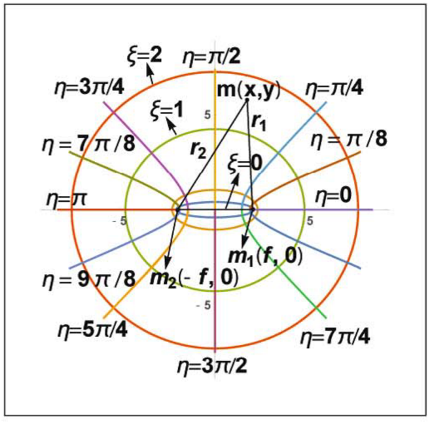
\includegraphics[width=0.5\textwidth]{Fig 2.png}
    \caption{the elliptical coordinate system $(\xi,\eta)$. Relative to polar coordinates, $\xi$ can be thought of as correspondent to radial distance $r$, and $\eta$ the angle $\theta$. Adopted from \cite{Krishnaswami2019}}.
    \label{fig:coordinatesys}
\end{figure}

Therefore, there are two conserved quantities in the system: Whittaker's constant (see \cite[p. 100]{Krishnaswami2019}) and total energy. Whittaker's constant can be represented as
\begin{equation}
    \begin{aligned}
        w & =\bm{L_1}\cdot\bm{L_2}+2mf(-\mu _1 \cos{\theta _1} +\mu _2 \cos{\theta _2})                           \\
          & =m^2r_1^2r_2^2\dot{\theta _1}^2\dot{\theta _2}^2+2mf(-\mu _1 \cos{\theta _1} +\mu _2 \cos{\theta _2}) \\
          & =-2mf^2E-\alpha
    \end{aligned}
\end{equation}
where $r_i$ is the distance $|\bm{r_i}-\bm{r}|$ between $m_i$ and $m$; $\bm{L_i}=mr_i^2\dot{\theta _i}\hat{z}$ is the angular momentum of a mass; $\theta _i$ is the angle between $\bm{r_i}$ and the $x$-axis; $\mu _i=Gmm_i$; and $\alpha$ is the “separation constant” derived from the separation of variables of $E$ in elliptical coordinates \cite[p. 101]{Krishnaswami2019}.

Since there are also just two degrees of freedom in this case, the system is exactly analytically solvable by integration in the Liouville sense. See Ó'Mathúna \cite[pages 49-105 and 113-142]{OMathuna2008} for a detailed solution.

\section{Numerical Solution}\label{sec:numerical}

\subsection{Finding Equations}\label{sec:equations}
While analytical solutions are useful for determining the exact motion of systems, numerical solutions are often much simpler. Such is the case here.
To do this, without loss of generality, shift the system so that $m_1$ is at the origin and $m_2$ is a distance $d$ along the $y$-axis from the origin. Now represent $m_2$ as a factor of $m_1=m_a$ such that $m_2=\alpha m_a$, as shown in Fig. \ref{fig:shiftedsys}.
\begin{figure}
    \centering
    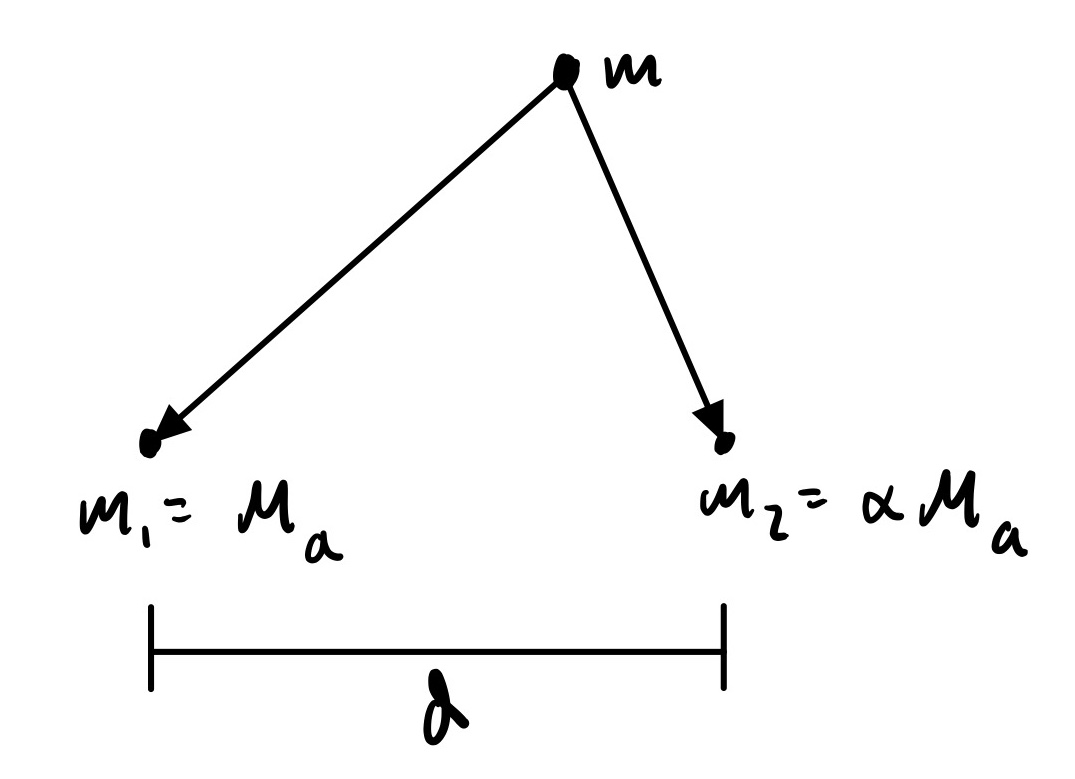
\includegraphics[width=0.5\textwidth]{Fig 3.jpeg}
    \caption{the shifted system with $m_1$ at the origin}
    \label{fig:shiftedsys}
\end{figure}

Up until this point, the masses and distances have been unitless and arbitrary. If these masses are instead measured in terms of solar units, further simplifications arise. If $m_a\equiv m_1$ is set to a “solar mass”, we see that $Gm_a=4\pi^2$. This is because the angular velocity of a mass around a primary (for example, the Earth around the Sun) is $2\pi*AU/yr$, where $AU$ is the average distance between the primary and the mass and $yr$ is the period (on Earth, one year). That is, the problem is nondimensionalized by setting the unit of mass to $m_1$ and the unit of time such that the period of the orbits of the primaries is $2\pi$ \cite{Wild1980,Worthington2012}.

Since the origin is now fixed, the equations of motion now use relative positioning to the origin (and $m_1$). From this and Newton's Law of Gravitation,
\begin{equation}
    \begin{aligned}
        F_x & =-\frac{Gm_a m}{r_1^3}x-\frac{G\alpha m_a m}{r_2^3}(x-d) \\
        F_y & =-\frac{Gm_a m}{r_1^3}y-\frac{G\alpha m_a m}{r_2^3}y
    \end{aligned}
    \label{eq:force}
\end{equation}
with $r_i=|\bm{r_i}-\bm{r}|$ the distance between $m$ and $m_i$. In cartesian coordinates, this results in
\begin{equation}
    \begin{aligned}
        \bm{r_1} & =x\hat{x}+y\hat{y}     \\
        \bm{r_2} & =(x-d)\hat{x}+y\hat{y}
    \end{aligned}
\end{equation}
so
\begin{equation}
    \begin{aligned}
        r_1 & =\sqrt{x^2+y^2}     \\
        r_2 & =\sqrt{(x-d)^2+y^2}
    \end{aligned}
\end{equation}

Plugging in $Gm_a=4\pi^2$ and dividing \ref{eq:force} by $m$ the following equations of acceleration emerge, dependent only on $x$ and $y$ positions
\begin{equation}
    \begin{aligned}
        \ddot{x}(x,y) & = 4\pi^2(\frac{x}{(x^2+y^2)^{\frac{3}{2}}}+\frac{\alpha(x-d)}{((x-d)^2+y^2)^{\frac{3}{2}}}) \\
        \ddot{y}(x,y) & = 4\pi^2y(\frac{1}{(x^2+y^2)^{\frac{3}{2}}}+\frac{\alpha}{((x-d)^2+y^2)^{\frac{3}{2}}})
    \end{aligned}
\end{equation}
This is a system of nonlinear differential equations. As demonstrated above, analytical solutions are possible, but messy.

\subsection{Plottable Solutions}
Instead of analytically solving this system, numerical integrators can be used. Here, Euler's Method, the Runge-Kutta 4\textsuperscript{th} Order Method, and the Forest \& Neri method will be demonstrated. There are many other methods that allow for approximate solutions of systems of coupled differential equations, such as the leapfrog method.

However, these particular methods have been chosen for several reasons. Euler's Method was chosen for its simplicity, speed, and ease of use with arrays (it accesses each element one-by-one). The Runge-Kutta 4\textsuperscript{th} Order Method was chosen because it is commonly used in general iterative differential equations solutions. Ther Forest \& Neri method was chosen because it was specifically written for use with force equations and computer modeling.

\subsubsection{Euler's Method}\label{sec:euler}
Euler's method is a simple and efficient formula to iteratively solve differential equations. Using Euler's approximation
\begin{equation}
    x(t+\delta t)=x(t)+\delta t\dot{x}(t)+O(\delta t^2)
    \label{eq:eulersmethod}
\end{equation}
and neglecting higher order terms $O(\delta t^2)$, the solution is quickly plottable in cartesian coordinates. The error (by which I mean local truncation error, or the potential error from each step) is on the order of $\delta t$ \cite[p. 298]{Wild1980}.
Adapting \ref{eq:eulersmethod} for $x$, $y$, $\dot{x}$, and $\dot{y}$, we get the following system of equations.
\begin{equation}
    \begin{aligned}
        x_{n+1}       & =x_n+\dot{x}_n\delta t                       \\
        y_{n+1}       & =y_n+\dot{y}_n\delta t                       \\
        \dot{x}_{n+1} & =\dot{x}_n-\delta t\ddot{x}(x_{n+1},y_{n+1}) \\
        \dot{y}_{n+1} & =\dot{y}_n-\delta t\ddot{y}(x_{n+1},y_{n+1})
    \end{aligned}
\end{equation}
When they are evaluated in order, this is an iterable, programmable, and plottable solution.

\subsubsection{Runge-Kutta Method}\label{sec:rungekutta}
Another way to incrementally solve integrable solutions is the Runge-Kutta method (specifically, the Runge-Kutta 4\textsuperscript{th} Order Method) \cite{Musielak_2014}. With the same logic of interation as the Euler Method above, Runge-Kutta allows for more precision by using intermediate steps to calculate the $n+1$ position. Runge-Kutta is much more precise than Euler's method, with an error of $O(\delta t^5)$. The general Runge-Kutta 4\textsuperscript{th} order method is \cite[p. 21]{Musielak_2014}:
\begin{equation}
    \begin{aligned}
        x_{n+1} & =x_n+\frac{1}{6}\delta t(k_1+2k_2+2k_3+k_4) \\
        k_1     & =f(x_n)                                     \\
        k_2     & =f(x_n+\delta t\frac{k_1}{2})               \\
        k_3     & =f(x_n+\delta t\frac{k_2}{2})               \\
        k_4     & =f(x_n+\delta tk_3)
    \end{aligned}
    \label{eq:rungekutta}
\end{equation}
Since both position and velocity can be calculated in this manner, in the context of this 3-Body problem, the equations become (evaluated in this order)
\begin{equation}
    \begin{aligned}
        x_{n+1}       & = x_n + \delta t\dot{x}_n                                                          \\
        y_{n+1}       & = y_n + \delta t\dot{y}_n                                                          \\
        {k_1}_x       & = \ddot{x}(x_{n+1},y_{n+1})                                                        \\
        {k_1}_y       & = \ddot{y}(x_{n+1},y_{n+1})                                                        \\
        {k_2}_x       & = \ddot{x}(x_{n+1}+ \delta t \frac{{k_1}_x}{2}, y_{n+1}+\delta t\frac{{k_1}_y}{2}) \\
        ...                                                                                                \\
        \dot{x}_{n+1} & = \dot{x}_n + \frac{1}{6}\delta t({k_1}_x+2{k_2}_x+2{k_2}_x+{k_4}_x)
    \end{aligned}
    \label{eq:rungekutta-3bp}
\end{equation}

\subsubsection{Forest \& Neri Method}\label{sec:forestneri}
The Forest and Neri method  is an alternative 4\textsuperscript{th} order integrator to the Runge-Kutta method that requires fewer calculations and is more precise \cite[pp. 60-61]{Kinoshita1990}. While the Runge-Kutta method is applicable to any numerical solution of a system of equations, Forest and Neri's method is specifically adapted to computer solutions to modeling force equations. The equations are as follows:
\begin{equation}
    \begin{aligned}
         & \beta=2^\frac{1}{3}, c_4=c_1=\frac{1}{2(2-\beta)}, c_3=c_2=\frac{1-\beta}{2(2-\beta)} \\
         & d_3=d_1=\frac{1}{2-\beta}, d_2=\frac{-\beta}{2-\beta}, d_4=0
    \end{aligned}
\end{equation}
\begin{equation}
    \begin{split}
        &x_1=x_n+ \delta tc_1 \dot{x}_n\\
        &x_2=x_1+ \delta tc_2 \dot{x}_1\\
        &...\\
        &x_{n+1}=x_4
    \end{split}
    \qquad(\text{for }x\text{ and } y)\qquad
    \begin{split}
        &\dot{x}_1=\dot{x}_n+\delta td_1\ddot{x}(x_1,y_1)\\
        &\dot{x}_2=\dot{x}_1+\delta td_2\ddot{x}(x_2,y_2)\\
        &...\\
        &\dot{x}_{n+1}=\dot{x}_4
    \end{split}
    \label{eq:forestandneri}
\end{equation}
As with Runge-Kutta, when calculated in order, this is an iterative solution. The error is on the order of $O(\delta t^5)$.

\section{Interpreting Solutions}\label{sec:description}
\begin{figure}
    \centering
    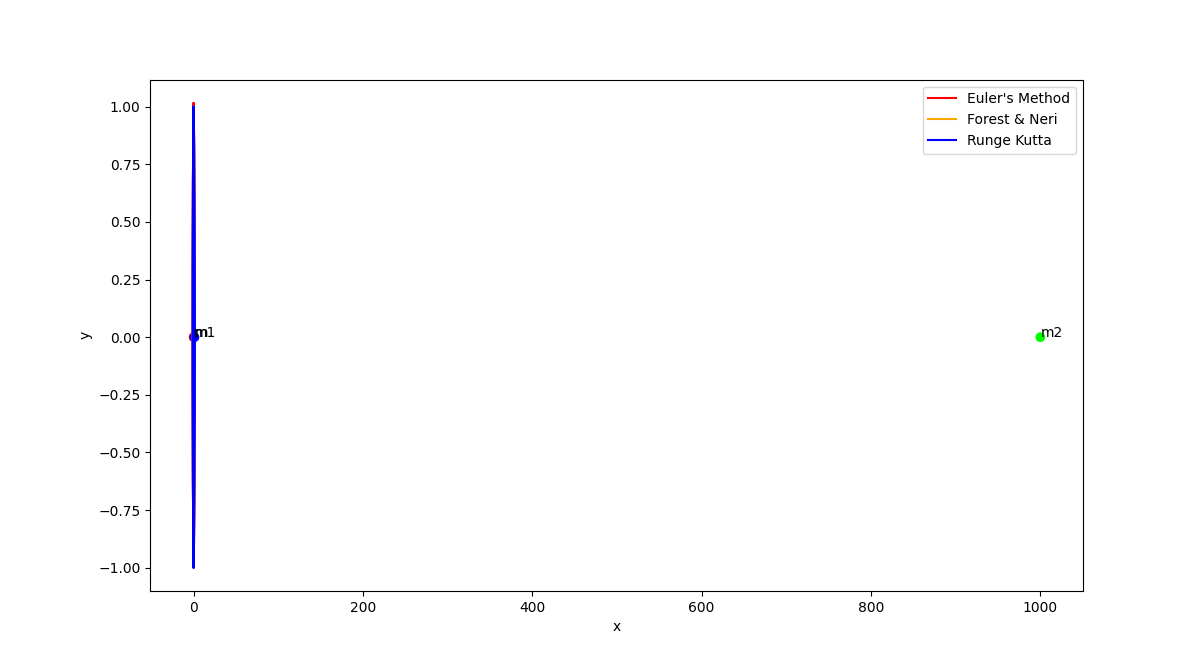
\includegraphics[width=0.49\textwidth]{Far M2.png}
    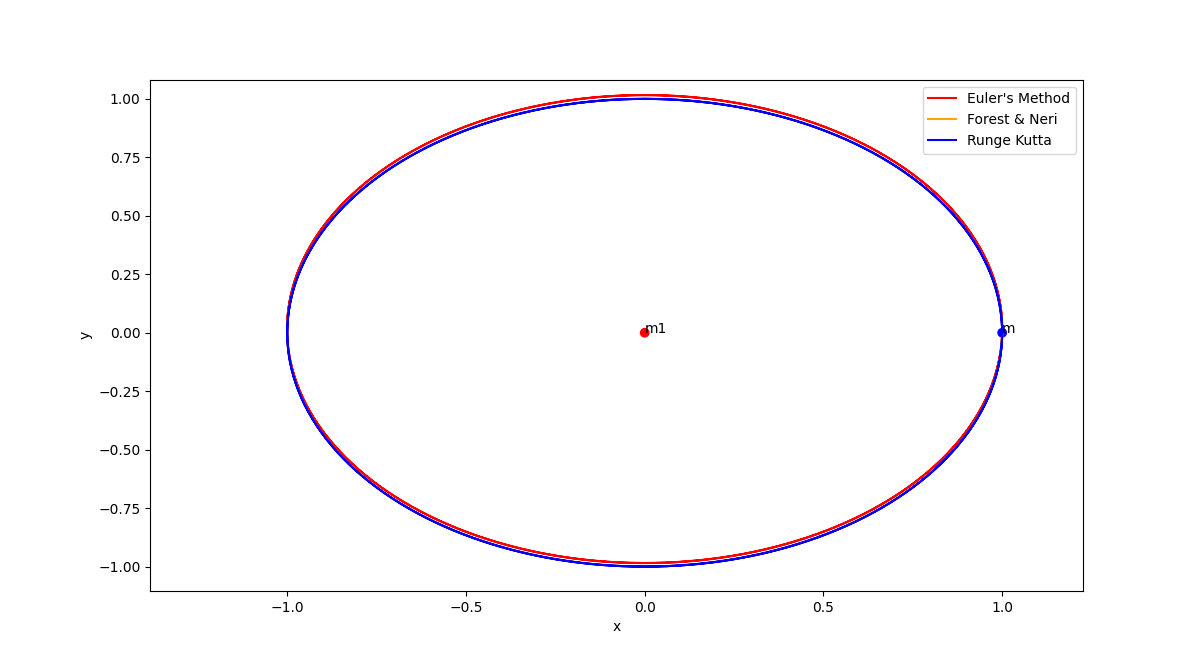
\includegraphics[width=0.49\textwidth]{Far M2 Zoomed.png}
    \caption{With a large $d$, the system behaves as though there is only one star. {\bf(Left)} The full system overview. {\bf(Right)} The same system, zoomed in to the moving mass.}
    \label{fig:farstar}
\end{figure}

\begin{figure}
    \centering
    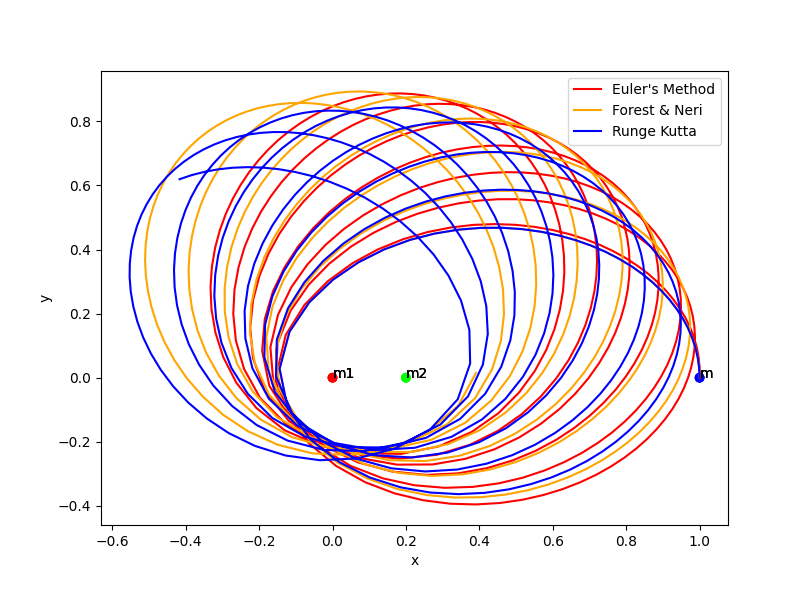
\includegraphics[width=0.49\textwidth]{Overlay 400 0.005.png}
    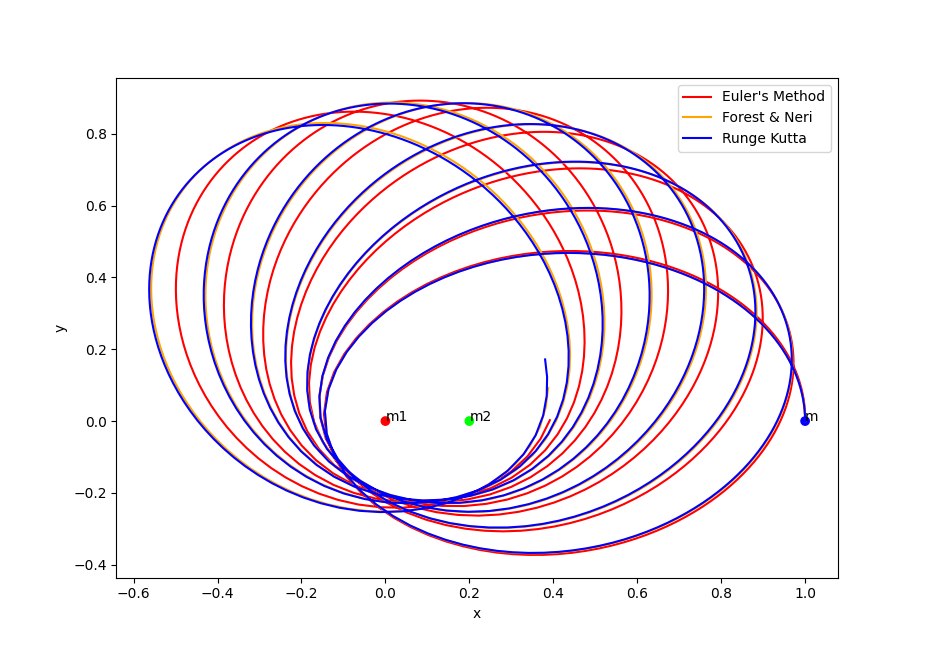
\includegraphics[width=0.49\textwidth]{Overlay 800 0.0025.png}
    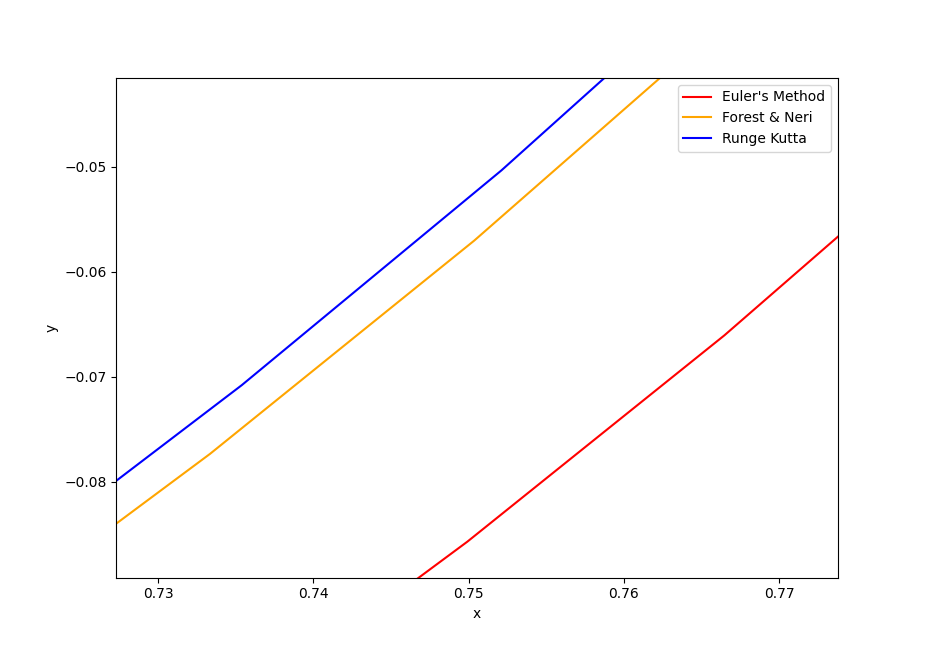
\includegraphics[width=0.49\textwidth]{Overlay 800 0.0025 Zoom.png}
    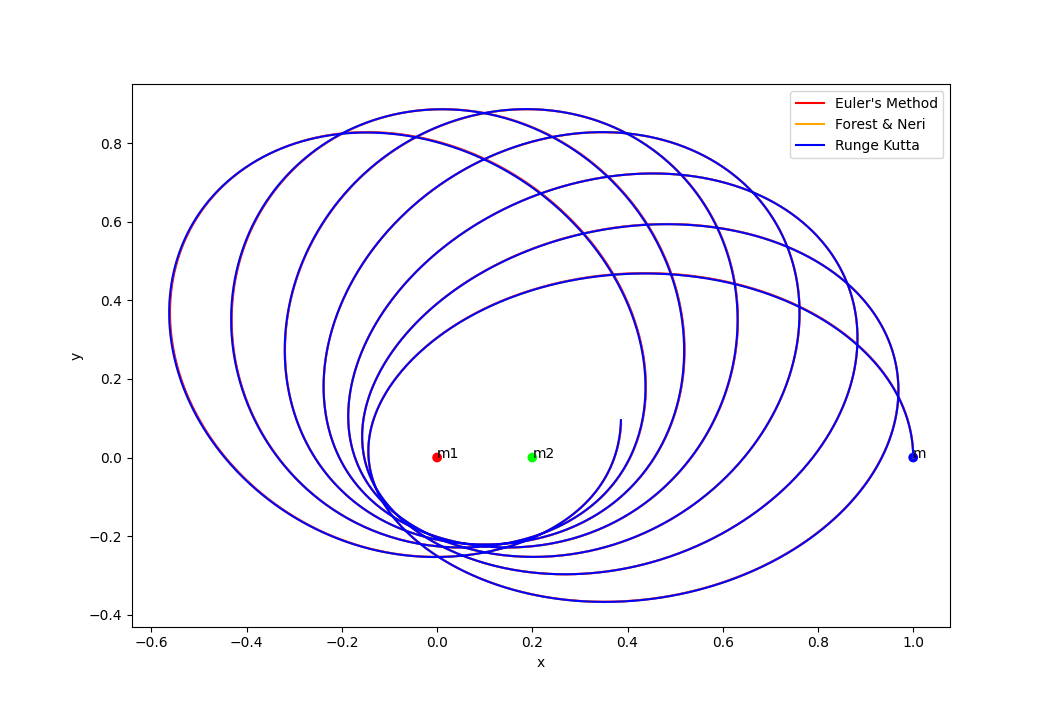
\includegraphics[width=0.49\textwidth]{Overlay 4000 0.0005.png}
    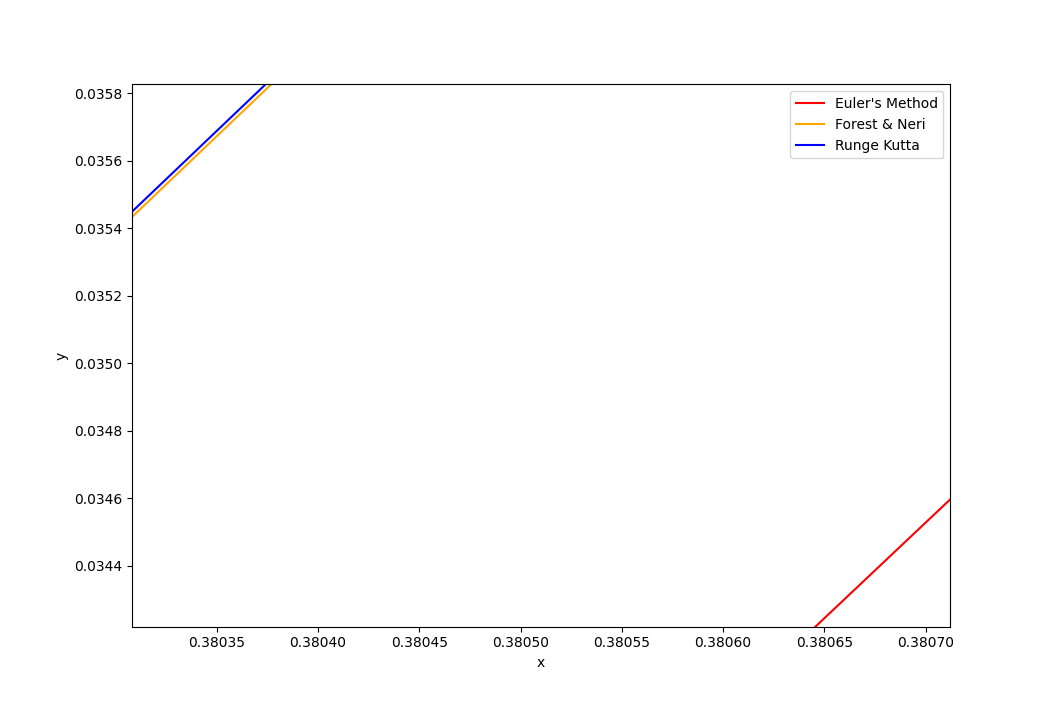
\includegraphics[width=0.5\textwidth]{Overlay 4000 0.0005 Zoom.png}
    \caption{All graphs are with the same initial conditions, but different iteration size.\\{\bf(Top Left)} Graph at $\delta t=0.005$. All three methods are noticably separated. {\bf(Top Right)} Graph at $\delta t=0.0025$ {\bf(Middle Left)} Zoomed in graph at $\delta t=0.0025$ to show difference between Forest \& Neri \ref{sec:forestneri} and Runge-Kutta \ref{sec:rungekutta} methods. Euler's method \ref{sec:euler} is still noticably different. {\bf(Middle Right)} Graph at $\delta t=0.0005$ {\bf(Bottom)} Zoomed in graph at $\delta t=0.0005$. All three methods are very close at this $\delta t$.}
    \label{fig:diffbetweenmethods}
\end{figure}


There are several cases in the limit where this solution demonstrates its clarity. The first case is when $d$ is very large (and $x$ is not) \ref{fig:farstar}. In this case, the terms dependent on $r_2$ disappear. This is equivalent to a system with only one star with mass $m_a$. On the other hand, if $d$ is very small, $r_1\approxeq r_2$. This is also equivalent to a system with one star, but this time the star has a mass $(1+\alpha)m_a$.

From Fig. \ref{fig:diffbetweenmethods}, we can see the difference between methods and iteration size. At large iteration size (higher error), the difference between the methods is far more pronounced. Indeed, the curves are noticably not smooth. As the errors compound, the final positions between the methods are very different. Decreasing the iteration size by a factor of 2 results in much closer results. In fact, it is hard at first glance to differentiate between the Runge-Kutta and Forest \& Neri methods -- only after zooming in is the difference evident. The closeness between the methods increases even further when $\delta t$ is decrease by another factor of 5. Here, even Euler's method is very similar to the 4\textsuperscript{th} order methods, although they are still closer to each other.


\appendix
\section{Code}\label{sec:code}
The code for this project is fully available at \href{https://github.com/jasperswallen/PHYS304-Project}{\color{blue}{\underline{my public GitHub repository}}},
containing both a Jupyter Notebook and command-line Python script. The requirements to run these are Python 3, \texttt{matplotlib}, and \texttt{numpy} (as well as \texttt{ipywidgets} for the Jupyter Notebook). Then, run \texttt{\$ python3 main.py} and input the initial positions and masses of all three objects, as well as the initial velocity of the moving object. Alternatively, use the \texttt{main.ipynb} Jupyter Notebook to input values from a browser or IDE. The Jupyter Notebook presentation of graphs is slightly different, as each method is in its own graph to show the evolution of the function with respect to time.

The following is \texttt{eulerMethod()}, which calculates and plots the graph of Euler's Three Body Problem with Euler's numerical approximation method. This code is found in \texttt{main.py} and \texttt{main.ipynb}.

\begin{lstlisting}[language=Python, numbers=left, breaklines=true]
def eulerMethod(moving_mass_x, moving_mass_y, moving_mass_x_prime, moving_mass_y_prime, its, delta):
    # declare arrays that will be appended to in loop
    x = [moving_mass_x]
    y = [moving_mass_y]
    x_prime = [moving_mass_x_prime]
    y_prime = [moving_mass_y_prime]

    for n in range(its):
        # calculate next x, y, x', and y'
        x_n_plus_one = x[n] + delta * x_prime[n]
        x.append(x_n_plus_one)
        y_n_plus_one = y[n] + delta * y_prime[n]
        y.append(y_n_plus_one)

        x_prime_n_plus_one = x_prime[n] + delta * \
            calculateXAccel(x[n + 1], y[n + 1])
        x_prime.append(x_prime_n_plus_one)

        y_prime_n_plus_one = y_prime[n] + delta * \
            calculateYAccel(x[n + 1], y[n + 1])
        y_prime.append(y_prime_n_plus_one)

    plt.plot(x, y, label="Euler's Method", color="red")
\end{lstlisting}

The Runge-Kutta and Forest \& Neri methods work in a similar manner, although they require many more calculations per iteration.

Note: the Jupyter Notebook uses an additional recipe, colorline \cite{Colorline}, to show evolution with time.

\bibliography{bibliography}

\end{document}
